

\documentclass[bigger]{beamer}

\usepackage{style}


\title[GRIN] %optional
{GRIN: Dead data elimination}

\subtitle{in the context of dependently typed languages}

\author[P. Podlovics, Cs. Hruska ] % (optional, for multiple authors)
{Péter Podlovics, Csaba Hruska, Andor Pénzes}

\institute[ELTE] % (optional)
{
	Eötvös Loránd University (ELTE), \\ Budapest, Hungary
}

\date{EUTypes-2019} % (optional)



\begin{document}
	
{
	\usebackgroundtemplate{
\includegraphics[width=\paperwidth]{title.jpg}}%
	\frame{\vspace{15mm}\titlepage}
}

\begin{frame}
	\frametitle{Overview}
	\tableofcontents
\end{frame}


\section{Introduction}

\begin{frame}[fragile]
	\frametitle{Why functional?}
	
	\begin{vfitemize}
		\item Declarativeness
			\begin{itemize}
				\item[pro:] can program on a higher abstraction level
			\end{itemize}
		\item Composability\\
			\begin{itemize}
				\item[pro:] can easily piece together smaller programs
				\item[con:] results in a lot of function calls
			\end{itemize}
		\item Functions are first class citizens
			\begin{itemize}
				\item[pro:] higher order functions
				\item[con:] unknown function calls
			\end{itemize}
	\end{vfitemize}

\end{frame}


\begin{frame}
\frametitle{Graph Reduction Intermediate Notation}

\begin{figure}[h]
	\centering
	\begin{adjustbox}{scale = 1.4}
		\tikzset{every loop/.style={-{Stealth[scale=1.5]}}}
		
		\begin{tikzpicture}[ node distance = 1.5cm and 1.5cm
		, on grid 
		, loop/.append style={-triangle 60}
		]
		
		\node [draw=black] (haskell)    									{Haskell};
		\node [draw=black] (idris)   [left  =of haskell]  {Idris};
		\node [draw=black] (agda)    [right =of haskell]  {Agda};
		\node [draw=black] (grin)    [below =of haskell]  {GRIN};
		\node [draw=black] (mc)      [below =of grin]     {Machine Code};
		
		\path[-{Stealth[scale=1.5]}] 
		(idris) edge [] (grin)
		(haskell) edge [] (grin)
		(agda) edge [] (grin)
		(grin) edge [] (mc);
		
		
		\end{tikzpicture}
	\end{adjustbox}
	\label{grin-backend}
\end{figure}
\end{frame}


\begin{frame}[fragile]
\frametitle{Front end code}

\begin{minipage}{0.35\textwidth}
	
	\begin{haskellcode}
		main = sum (upto 0 10)
		
		upto n m
		  | n > m = []
		  | otherwise = n : upto (n+1) m
		
		sum []     = 0
		sum (x:xs) = x + sum xs
	\end{haskellcode}
\end{minipage}
\hfill 
\pause
\begin{minipage}{0.4\textwidth}
	\vspace{2cm}
	\begin{figure}[h]
		\centering
		\begin{adjustbox}{scale = 1.4}
			\tikzset{every loop/.style={-{Stealth[scale=1.5]}}}
			
			\begin{tikzpicture}[ node distance = 1.3cm and 1cm
			, on grid 
			, loop/.append style={-triangle 60}
			]
			
			\node [shape=ellipse,draw=black] (main)                        {main};
			\node [shape=ellipse,draw=black] (eval) [below =of main]       {eval};
			\node [shape=ellipse,draw=black] (sum)  [below left =of eval]  {sum};
			\node [shape=ellipse,draw=black] (upto) [below right =of eval] {upto};
			
			\path[-{Stealth[scale=1.5]}] 
			(main) edge [] (eval)
			(eval) edge [bend left] (sum)
			(eval) edge [bend right] (upto)
			(sum) edge [bend left] (eval)
			(upto) edge [bend right] (eval);
			
			
			\end{tikzpicture}
		\end{adjustbox}
		\label{control-flow-lazy}
	\end{figure}
\end{minipage}
\end{frame}


\begin{frame}[fragile]
\frametitle{GRIN code}

\begin{minipage}{0.4\textwidth}
	
	\begin{haskellcode}
		grinMain = 
		  t1 <- store (CInt 1)
		  t2 <- store (CInt 10)
		  t3 <- store (Fupto t1 t2)
		  t4 <- store (Fsum t3)
		  (CInt r) <- eval t4
		  _prim_int_print r
	\end{haskellcode}
\end{minipage}
\hfill
\begin{minipage}{0.48\textwidth}
	\vspace{1cm}
	\begin{haskellcode}
		eval p = 
		  v <- fetch p
		  case v of
		    (CInt n)     -> pure v
		    (CNil)       -> pure v
		    (CCons y ys) -> pure v
		    (Fupto a b) -> 
		      zs <- upto a b
		      update p zs
		      pure zs
		    (Fsum c) -> 
		      s <- sum c
		      update p s
		      pure s
	\end{haskellcode}
\end{minipage}


\end{frame}


\begin{frame}[fragile]
\frametitle{Transformation machinery}

	\begin{vfitemize}
		
		\item Inline calls to \mintinline{haskell}{eval}
		\item Run dataflow analyses:
			\begin{itemize}
				\item Heap points-to analysis
				\item Sharing analysis
			\end{itemize}
		\item Run transformations until we reach a fixed-point:
			\begin{itemize}
				\item Sparse Case Optimization
				\item Common Subexpression Elimination
				\item Generalized Unboxing
				\item etc \dots
			\end{itemize}
		
	\end{vfitemize}


\end{frame}


\section{Extensions}

\begin{frame}[fragile]
\frametitle{Extending Heap points-to}

	\vspace{1cm}
	\begin{minipage}{\textwidth}
		\begin{figure}
			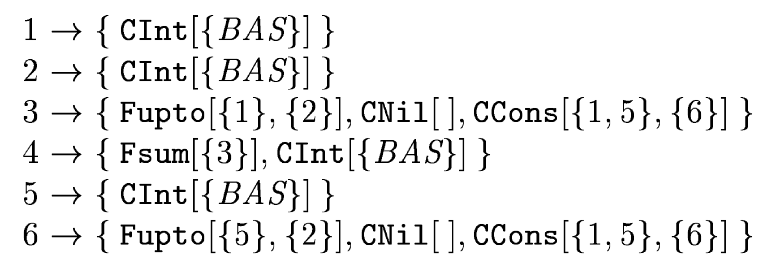
\includegraphics[scale=0.3]{hpt-boq.png}
		\end{figure}
	\end{minipage}
	\vfill
	\pause
	\begin{minipage}{\textwidth}
		\begin{figure}
			$BAS \in \{ \text{Int64}, \text{Float}, \text{Bool}, \text{String}, \text{Char} \}$
		\end{figure}
	\end{minipage}
	\vfill
	\pause
	\begin{center}
		\begin{minipage}{0.8\textwidth}
			% real type would be: a -> State# s -> (# State# s, MutVar# s a #)
			\begin{haskellcode}
				indexArray# :: Array# a -> Int# -> (# a #)
				newMutVar#  :: a -> s -> (# s, MutVar# s a #)
			\end{haskellcode}
		\end{minipage}
	\end{center}

\end{frame}


\begin{frame}[fragile]
\frametitle{LLVM back end}

	\hspace{-4cm}
	\begin{minipage}[t]{0.30\textwidth}
		\begin{minted}[fontsize=\scriptsize]{haskell}		
			grinMain =
			 t1 <- store (CInt 1)
			 t2 <- store (CInt 10)
			 t3 <- store (Fupto t1 t2)
			 t4 <- store (Fsum t3)
			 (CInt r') <- eval t4
			 _prim_int_print r'
			 
			upto m n =
			 (CInt m') <- eval m
			 (CInt n') <- eval n
			 b' <- _prim_int_gt m' n'
			 case b' of
			   #True -> pure (CNil)
			   
			sum l = ...
			
			eval p = ...
		\end{minted}
	\end{minipage}
	\hspace{1.8cm}
	\pause
	\begin{minipage}[t]{0.30\textwidth}
		\begin{minted}[fontsize=\scriptsize]{haskell}
		grinMain =
		 n1 <- sum 0 1 10
		 _prim_int_print n1
		
		sum s lo hi =
		 b <- _prim_int_gt lo hi
		 if b then
		  pure s
		 else
		  lo' <- _prim_int_add lo 1
		  s' <- _prim_int_add s lo
		  sum s' lo' hi

		\end{minted}
	\end{minipage}
	\hspace{0.5cm}
	\pause
	\begin{minipage}[t]{0.30\textwidth}
		\begin{minted}[fontsize=\scriptsize]{asm}
		grinMain:                      
		# BB#0:                     
		  movabsq    $55, %rdi  
		  jmp    _prim_int_print       
		\end{minted}
	\end{minipage}

\end{frame}
%$

\section{Dead Data Elimination}

\begin{frame}[fragile]
\frametitle{Dead data elimination I.}

\begin{center}
	\begin{minipage}{0.30\textwidth}
		\begin{haskellcode}
			length : List a -> Nat
			length Nil = Z
			length (Cons x xs) 
			  = S (length xs)
		\end{haskellcode}
	\end{minipage}
	\hspace{1cm}
	$\xRightarrow{\text{DDE}}$
	\hfill
	\begin{minipage}{0.5\textwidth}
		\begin{haskellcode}
			length p =
			 xs <- fetch p
			 case xs of
			  (Cons ys) ->
			   l1 <- length ys
			   l2 <- _prim_int_add l1 1
			   pure l2
			  (Nil) ->
			    pure 0
		\end{haskellcode}
	\end{minipage}
\end{center}

\end{frame}


\begin{frame}[fragile]
\frametitle{Dead data elimination II.}

\begin{center}
	\begin{minipage}{0.85\textwidth}
		\begin{haskellcode}
			data Bin : Nat -> Type where
			  N : Bin 0
			  O : {n : Nat} -> Bin n -> Bin (2*n + 0)
			  I : {n : Nat} -> Bin n -> Bin (2*n + 1)
		\end{haskellcode}
		\vspace{0.5cm}
		\pause
		\begin{haskellcode}
			binToNat : Bin n -> Nat
			binToNat N = 0
			binToNat (O {n} _) = 2*n
			binToNat (I {n} _) = 2*n + 1
		\end{haskellcode}
	\end{minipage}
\end{center}

\end{frame}


\begin{frame}
\frametitle{Applications}

	\begin{vfitemize}
		\item Map $\rightarrow$ Set
		\item Type class dictionaries
		\item Type erasure for dependently typed languages
	\end{vfitemize}

\end{frame} 

\begin{frame}
\frametitle{What do we need?}

	\begin{vfitemize}
		\item Producers \& consumers
		\item Detect dead fields
		\item Connect consumers to producer
		\item Remove or transform dead fields
	\end{vfitemize}

\end{frame}


\begin{frame}[fragile]
\frametitle{Created-by}

\begin{center}
	\begin{minipage}{0.50\textwidth}
		\begin{haskellcode}
			null xs = 
			 y <- case xs of
			  (CNil) -> 
			   a <- pure (CTrue)
			   pure a
			  (CCons z zs) ->
			   b <- pure (CFalse)
			   pure b
			 pure y 
		\end{haskellcode}
	\end{minipage}
	\hfill
	\begin{minipage}{0.475\textwidth}
		\begin{tcolorbox}[tab2,tabularx={l|r}]
			Var			        & Producers \\
			\hline\hline
			\pilcode{xs}    & $CNil[\dots], CCons[\dots]$ \\\hline
			\pilcode{a}     & $CTrue[\pilcode{a}]$	\\\hline
			\pilcode{b}     & $CFalse[\pilcode{b}]$ \\\hline
			\pilcode{y}     & $CTrue[\pilcode{a}], CFalse[\pilcode{b}]$ \\
		\end{tcolorbox}
	\end{minipage}
\end{center}

\end{frame}


\begin{frame}
\frametitle{Producers and consumers}

\begin{figure}[h]
\centering
\begin{adjustbox}{scale = 1.3}
	\begin{tikzpicture}[ node distance = 1cm and 2cm, on grid ]
	
	\node<1> [shape=circle,draw=black] (P1)                 {$P_1$};
	\node<1> [shape=circle,draw=black] (P2) [right =of P1]  {$P_2$};
	\coordinate (Middle) at ($(P1)!0.5!(P2)$);
	\node<1> [shape=circle,draw=black] (C2) [below =of Middle]  {$C_2$};
	\node<1> [shape=circle,draw=black] (C1) [left =of C2]       {$C_1$};
	\node<1> [shape=circle,draw=black] (C3) [right =of C2]      {$C_3$};
	
	\path<1>[-{Stealth[scale=1.5]}] (P1) edge [] (C1)
	(P1) edge [] (C2)
	(P2) edge [] (C2)
	(P2) edge [] (C3);
	
	\pause
	
	\node<2,3,4> [shape=circle,draw=black] (P1)                 {\pilcode{upto}};
	\node [shape=circle,draw=black] (P2) [right =of P1]  {\pilcode{upto}};
	\coordinate (Middle) at ($(P1)!0.5!(P2)$);
	\node<2> [shape=circle,draw=black] (C2) [below =of Middle]  {\pilcode{len}};
	\node<2> [shape=circle,draw=black] (C1) [left =of C2]       {\pilcode{len}};
	\node<2,3,4,5> [shape=circle,draw=black] (C3) [right =of C2]      {\pilcode{sum}};
	
	\path[-{Stealth[scale=1.5]}] (P1) edge [] (C1)
	(P1) edge [] (C2)
	(P2) edge [] (C2)
	(P2) edge [] (C3);
	
	\pause 
	
	\node<3> [shape=circle,draw=black,fill=green] (C2) [below =of Middle]  {\pilcode{len}};
	\node<3> [shape=circle,draw=black,fill=green] (C1) [left =of C2]       {\pilcode{len}};
	\node<3> [shape=circle,draw=black,fill=red]   (C3) [right =of C2]      {\pilcode{sum}};
	
	\pause 
	
	\node<4,5,6,7,8,9> [shape=circle,draw=black,dashed] (C2) [below =of Middle]  {\pilcode{len}};
	\node<4,5,6,7,8,9> [shape=circle,draw=black,dashed] (C1) [left =of C2]       {\pilcode{len}};
	
	\pause
	
	\node<5,6,7,8,9> [shape=circle,draw=black,dashed] (P1)                 {\pilcode{upto}};
		
	\pause
	
	\node<6,7,8,9> [shape=circle,draw=black,fill=lightgray]   (C3) [right =of C2]      {\pilcode{sum}};
	
	\pause 
	
	\node<7,8,9> [shape=circle,draw=black,fill=lightgray] (P2) [right =of P1]  {\pilcode{upto}};
	
	\pause 
	
	\node<8> [shape=circle,draw=black,dashed,fill=lightgray] (C2) [below =of Middle]  {\pilcode{len}};
	
	\pause 
	
	\node<9> [shape=circle,draw=black,dashed,fill=lightgray] (C2) [below =of Middle]  {\pilcode{len}\Lightning};
	
	\pause
	
	% first solution is not doing anything
	
	\node<10> [shape=circle,draw=black,fill=lightgray] (P1)                 {\pilcode{upto}};
	\node<10,11> [shape=circle,draw=black,fill=lightgray] (P2) [right =of P1]  {\pilcode{upto}};
	\node<10,11> [shape=circle,draw=black,fill=lightgray] (C2) [below =of Middle]  {\pilcode{len}};
	\node<10,11> [shape=circle,draw=black,fill=lightgray] (C1) [left =of C2]       {\pilcode{len}};
	\node<10,11> [shape=circle,draw=black,fill=lightgray]   (C3) [right =of C2]      {\pilcode{sum}};
	
	\pause 
	
	% second solution is to keep each C & P's structure as it is, but dummify P1
	
	\node<11> [shape=circle,draw=black,fill=yellow] (P1)                 {\pilcode{upto}};
	
	\pause
	
	% third solution is to restructure C2, but keep the original pattern as well (code duplication, needs IR improvement)
	
	\node<12> [shape=circle,draw=black,dashed] (P1)                 {\pilcode{upto}};
	\node<12> [shape=circle,draw=black,fill=lightgray] (P2) [right =of P1]  {\pilcode{upto}};
	
	\node<12> [shape=circle,draw=black,pattern=north east lines, dashed] (C2) [below =of Middle]  {\pilcode{len}};
	\node<12> [shape=circle,draw=black,dashed] (C1) [left =of C2]       {\pilcode{len}};
	\node<12> [shape=circle,draw=black,fill=lightgray] (C3) [right =of C2]      {\pilcode{sum}};
	
	
	
	
	\end{tikzpicture}
\end{adjustbox}
\label{fig:producers-and-consumers}
\end{figure}

\end{frame}



\section{Results}

\begin{frame}[fragile]
\frametitle{Setup}

	\vspace{1.5cm}
	\begin{vfitemize}
		\item Small Idris code snippets from: \\
		\textit{Type-driven Development with Idris} by Edwin Brady
		\item Only interpreted code
		\item Compile- \& runtime measurements
		\item Pipeline setup:	
	\end{vfitemize}

	\begin{figure}
		\begin{adjustbox}{scale = 1}
			\tikzset{every loop/.style={-{Stealth[scale=1.5]}}}
			
			%\hspace{-1cm}
			\begin{tikzpicture}[ node distance = 1.5cm and 3cm
			, on grid 
			, loop/.append style={-triangle 60}
			]
			
			\node [draw=black] (cg)    									{Code gen.};
			\node [draw=black] (ro1) [right =of cg]  {Regular Opts.};
			\node [draw=black] (dde) [right =2.5cm of ro1]  {DDE};
			\node [draw=black] (ro2) [right =2.5cm of dde]  {Regular Opts.};
			
			\path[-{Stealth[scale=1.5]}] 
			(cg) edge [] (ro1)
			(ro1) edge [loop] (ro1)
			(ro1) edge [] (dde)
			(dde) edge [] (ro2)
			(ro2) edge [loop] (ro2);
			
			
			\end{tikzpicture}
		\end{adjustbox}
		\label{fig:-measurement-pipeline}
	\end{figure}

\end{frame}



\begin{frame}[fragile]
\frametitle{Length}
	% real example
	
	\begin{figure}
		\hspace{-1cm}
		\begin{minipage}{0.45\textwidth}
			\resizebox{\width}{5.5cm}{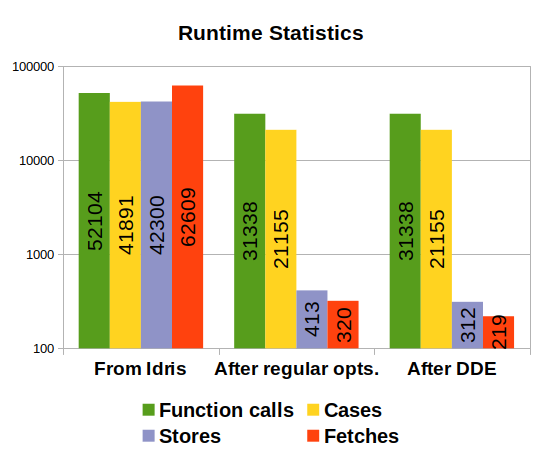
\includegraphics[scale=0.40]{length_rt.png}}
		\end{minipage}
		\hspace{1cm}
		\begin{minipage}{0.45\textwidth}
			\resizebox{\width}{5.5cm}{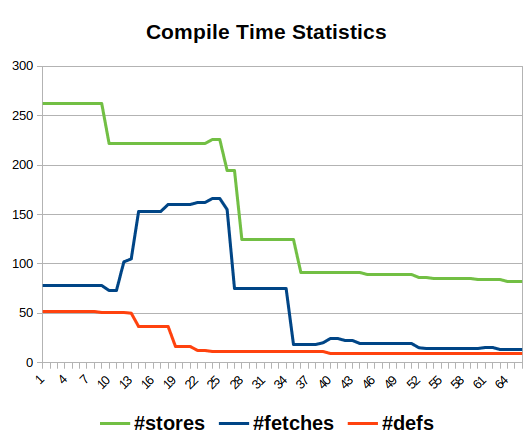
\includegraphics[scale=0.40]{length_ct.png}}
		\end{minipage}
	\end{figure}
	
\end{frame}

\begin{frame}[fragile]
\frametitle{Exact length}
	% no stores & no fetches! (Maybe transformed)
	\begin{figure}
		\hspace{-1cm}
		\begin{minipage}{0.45\textwidth}
			\resizebox{\width}{5.5cm}{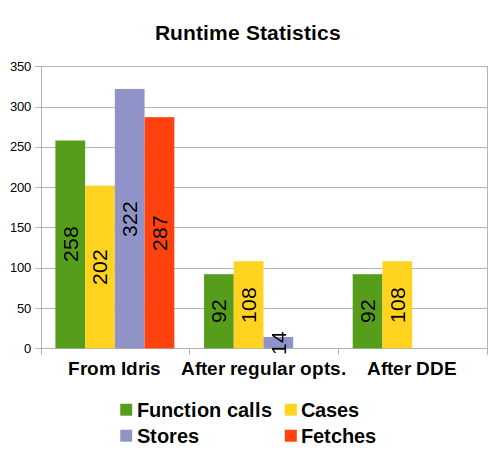
\includegraphics[scale=0.40]{exact_length_rt.png}}
		\end{minipage}
		\hspace{1cm}
		\begin{minipage}{0.45\textwidth}
			\resizebox{\width}{5.5cm}{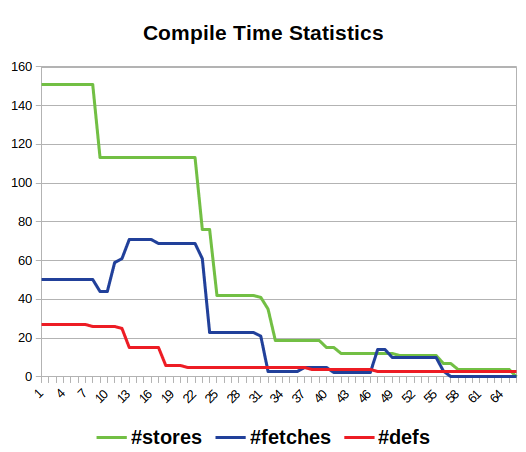
\includegraphics[scale=0.40]{exact_length_ct.png}}
		\end{minipage}
	\end{figure}
\end{frame}

\begin{frame}[fragile]
\frametitle{Reverse}
  % interesting example, but no DDE
  \begin{figure}
  	\hspace{-1cm}
  	\begin{minipage}{0.45\textwidth}
  		\resizebox{\width}{5.5cm}{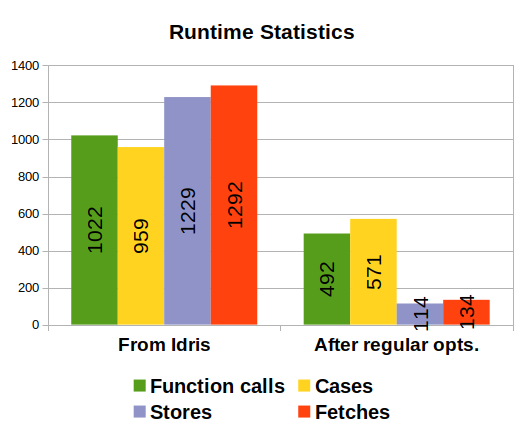
\includegraphics[scale=0.40]{reverse_rt.png}}
  	\end{minipage}
  	\hspace{1cm}
  	\begin{minipage}{0.45\textwidth}
  		\resizebox{\width}{5.5cm}{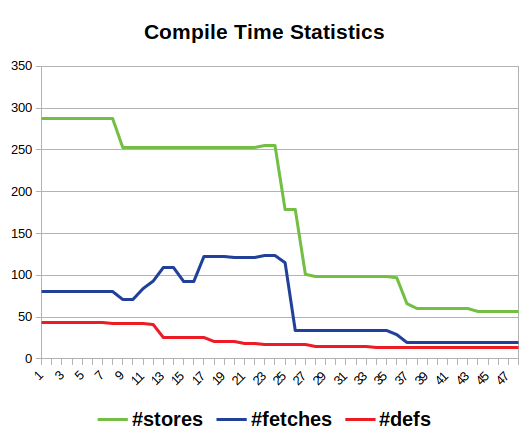
\includegraphics[scale=0.40]{reverse_ct.png}}
  	\end{minipage}
  \end{figure}
\end{frame}

\begin{frame}[fragile]
\frametitle{Type level functions}
  % caveat
  \begin{figure}
  	\hspace{-1cm}
  	\begin{minipage}{0.45\textwidth}
  		\resizebox{\width}{5.5cm}{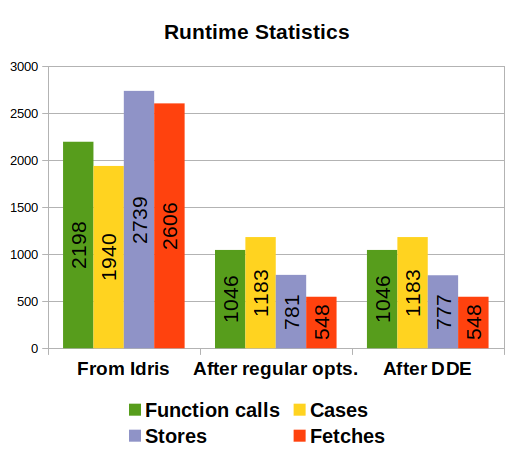
\includegraphics[scale=0.40]{tyfuns_rt.png}}
  	\end{minipage}
  	\hspace{1cm}
  	\begin{minipage}{0.45\textwidth}
  		\resizebox{\width}{5.5cm}{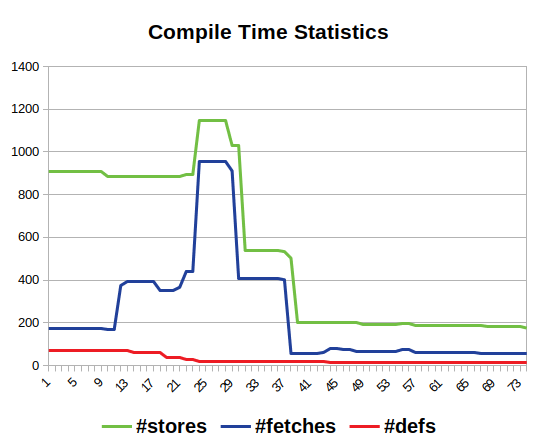
\includegraphics[scale=0.40]{tyfuns_ct.png}}
  	\end{minipage}
  \end{figure}
\end{frame}


\begin{frame}[fragile]
\frametitle{Conclusions}
	\begin{vfitemize}
		\item The optimizer works well:
			\begin{itemize}
				\item the number of stores, fetches, function calls and pattern matches significantly decreased
				\item the structure of the code resembles that of an imperative language
			\end{itemize}
		\item Dead Data Elimination:
			\begin{itemize}
				\item is a bit costly 
				\item is a specific optimization
				\item can completely transform data structures
				\item can trigger further transformations
			\end{itemize}
	\end{vfitemize}
\end{frame}


{
	\usebackgroundtemplate{
\includegraphics[width=\paperwidth]{title.jpg}}%
	\begin{frame}{}
	
	\bigskip\bigskip\bigskip
	
	{\bf\Huge\color{white} THANK YOU}
	
	\bigskip
	
	{\bf\Huge\color{white} FOR YOUR}
	
	\bigskip
	
	{\bf\Huge\color{white} ATTENTION!}
	
\end{frame}
}

% Q&A

\begin{frame}[fragile]
\frametitle{Sparse case optimization}

\begin{center}
	\begin{minipage}{0.40\textwidth}
		\begin{haskellcode}
			<m0>
			v <- eval l
			case v of
			CNil       -> <m1>
			CCons x xs -> <m2>
		\end{haskellcode}
	\end{minipage}
	$\xRightarrow{v \in \{ \text{CCons}\}}$
	\hfill
	\begin{minipage}{0.40\textwidth}
		\begin{haskellcode}
			<m0>
			v <- eval l
			case v of
			CCons x xs -> <m2>
		\end{haskellcode}
	\end{minipage}
\end{center}

\end{frame}


\begin{frame}
\frametitle{Compiled data flow analysis}

\begin{vfitemize}
	\item Analyzing the syntax tree has an interpretation overhead
	\item We can work around this by "compiling" our analysis into an executable program
	\item The compiled abstract program is independent of the AST
	\item It can be executed in a different context (ie.: by another program or on GPU)
	\item After run (iteratively), it produces the result of the given analysis
\end{vfitemize}
\end{frame}



\end{document}

